\chapterauthor{Raphaël Couturier}{Femto-ST Institute, University of Franche-Comte}


\chapter{Presentation of the GPU architecture and of the Cuda environment}
\label{chapter1}

\section{Introduction}\label{ch1:intro}

This chapter introduces the Graphics  Processing Unit (GPU) architecture and all
the concepts needed to understand how GPUs  work and can be used to speed up the
execution of some algorithms. First of all this chapter gives a brief history of
the development  of Graphics  card until they  have been  used in order  to make
general   purpose   computation.    Then   the   architecture  of   a   GPU   is
illustrated.  There  are  many  fundamental  differences between  a  GPU  and  a
tradition  processor. In  order  to benefit  from the  power  of a  GPU, a  Cuda
programmer needs to use threads. They have some particularities which enable the
Cuda model to be efficient and scalable when some constraints are addressed.



\section{Brief history of Video Card}

Video  cards or Graphics  cards have  been introduced  in personal  computers to
produce  high quality graphics  faster than  classical Central  Processing Units
(CPU) and  to alleviate CPU from this  task. In general, display  tasks are very
repetitive and very specific.  Hence,  some manufacturers have produced more and
more sophisticated video cards, providing 2D accelerations then 3D accelerations,
then some  light transforms. Video cards  own their own memory  to perform their
computation.  For at least two decades, every personal computer has had a video
card which is simple for  desktop computers or which provides many accelerations
for game and/or  graphic oriented computers.  In the  latter case, graphic cards
may be more expensive than a CPU.

Since  2000, video  cards have  allowed  users to  apply arithmetic  operations
simultaneously on a sequence of  pixels, also later called stream processing. In
this case, the information of the pixels (color, location and other information) are
combined in order  to produce a pixel  color that can be displayed  on a screen.
Simultaneous  computations are  provided  by shaders  which calculate  rendering
effects on  graphics hardware with a  high degree of  flexibility. These shaders
handles the stream data with pipelines.


Some researchers  tried to  apply those operations  on other  data, representing
something different  from pixels,  and consequently this  resulted in  the first
uses of video cards for  performing general purpose computation. The programming
model  was not  easy  to use  at  all and  was very  dependent  of the  hardware
constraints.   More precisely  it consisted  in using  either DirectX  of OpenGL
functions  providing  an  interface  to  some classical  operations  for  videos
operations  (memory  transfers,  texture  manipulation,  ...).   Floating  point
operations were  most of the  time unimaginable.  Obviously when  something went
wrong, programmers had no way (and neither the tools) to detect it.

\section{GPGPU}

In order  to benefit from the computing  power of more recent  video cards, Cuda
was first proposed in 2007 by  NVidia. It unifies the programming model for some
of  their most performant  video cards.   Cuda~\cite{ch1:cuda} has  quickly been
considered by  the scientific community as  a great advance  for general purpose
graphics processing unit (GPGPU)  computing.  Of course other programming models
have been  proposed. The  other well-known alternative  is OpenCL which  aims at
proposing an alternative to Cuda  and which is multi-platform and portable. This
is a  great advantage since  it is even  possible to execute OpenCL  programs on
traditional CPUs.  The main drawback is that it is less tight with the hardware
and  consequently sometimes  provides  less efficient  programs. Moreover,  Cuda
benefits from  more mature compilation and optimization  procedures.  Other less
known environments  have been proposed, but  most of them have  been stopped, for
example  we can  cite: FireStream  by ATI  which is  not maintained  anymore and
replaced by  OpenCL, BrookGPU by  Standford University~\cite{ch1:Buck:2004:BGS}.
Another environment based  on pragma (insertion of pragma  directives inside the
code to  help the compiler to generate  efficient code) is call  OpenACC.  For a
comparison with OpenCL, interested readers may refer to~\cite{ch1:CMR:12}.



\section{Architecture of current GPUs}

The architecture  \index{architecture of  a GPU} of  current GPUs  is constantly
evolving.  Nevertheless  some trends remain constant  throughout this evolution.
Processing units composing a GPU are  far more simple than a traditional CPU but
it is much easier to integrate many computing units inside a GPU card than to do
so with many cores inside a CPU. This is due to the fact that the cores of a GPU are
simpler than the cores of a CPU.  In  2012, the most powerful GPUs own more than 500
cores       and       the       most       powerful      CPUs       have       8
cores. Figure~\ref{ch1:fig:comparison_cpu_gpu} shows  the number of cores inside
a  CPU  and  inside a  GPU.   In  fact,  in  a  current NVidia  GPU,  there  are
multiprocessors which have 32 cores (for example on Fermi cards). The core clock
of CPU is  generally around 3GHz and  the one of GPU is  about 1.5GHz.  Although
the core clock of GPU cores is slower, the amount of cores inside a GPU provides
more computational power.  This measure is commonly represented by the number of
floating point operation  per seconds. Nowadays the most powerful  GPUs provide more
than   1TFlops,  i.e.    $10^{12}$   floating  point   operations  per   second.
Nevertheless  GPUs are very  efficient to  perform some  operations but  not all
kinds of operations. They are very efficient to execute repetitive work in which
only  the data  change. It  is important  to keep  in mind  that multiprocessors
inside a GPU have 32 cores. Later we will see that these 32 cores need to do the
same work to get maximum performance.

\begin{figure}[b!]
\centerline{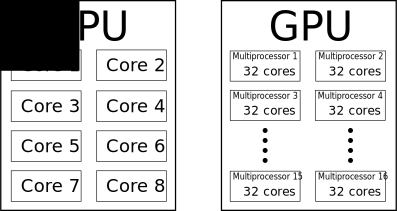
\includegraphics[]{Chapters/chapter1/figures/nb_cores_CPU_GPU.pdf}}
\caption{Comparison of number of cores in a CPU and in a GPU.}
%[Comparison of number of cores in a CPU and in a GPU]
\label{ch1:fig:comparison_cpu_gpu}
\end{figure}

On the most powerful  GPU cards, called Fermi, multiprocessors  are called streaming
multiprocessors  (SM). Each  SM contains  32  cores and  is able  to perform  32
floating points or integer operations on  32 bits numbers per clock or 16 floating
points  on  64 bits number  per  clock. SMs  have  their  own registers,  execution
pipelines and caches.  On Fermi architecture,  there are 64Kb shared memory + L1
cache  and 32,536 32bits  registers per  SM. More  precisely the  programmer can
decide what amount  of shared memory and  L1 cache SM can use.  The constraint is
that the sum of both amounts should be less or equal to 64Kb.

Threads are used to  benefit from the important number of cores  of a GPU. Those
threads    are   different    from    traditional   threads    for   CPU.     In
chapter~\ref{chapter2},  some  examples of  GPU  programming  will explicit  the
details of  the GPU  threads. However,  threads are gathered  into blocks  of 32
threads, called ``warps''. Those warps  are important when designing an algorithm
for GPU.


Another big  difference between CPU and GPU  is the latency of  memory.  In CPU,
everything is optimized  to obtain a low latency  architecture. This is possible
through  the  use  of  cache  memories. Moreover,  nowadays  CPUs  perform  many
performance optimizations  such as speculative execution  which roughly speaking
consists in executing  a small part of  code in advance even if  later this work
reveals itself  to be  useless. On the  contrary, GPUs  do not have  low latency
memory.   In comparison GPUs  have small  cache memories.  Nevertheless the
architecture of GPUs is optimized  for throughput computation and it takes into
account the memory latency.



\begin{figure}[b!]
\centerline{\includegraphics[scale=0.7]{Chapters/chapter1/figures/low_latency_vs_high_throughput.pdf}}
\caption{Comparison of low latency of CPU and high throughput of GPU.}
\label{ch1:fig:latency_throughput}
\end{figure}

Figure~\ref{ch1:fig:latency_throughput}  illustrates   the  main  difference  of
memory latency between a CPU and a  GPU. In a CPU, tasks ``ti'' are executed one
by one with a short memory latency to get the data to process. After some tasks,
there is  a context switch  that allows the  CPU to run  concurrent applications
and/or multi-threaded  applications. Memory latencies  are longer in a  GPU, the
the  principle  to   obtain  a  high  throughput  is  to   have  many  tasks  to
compute. Later we  will see that those tasks are called  threads with Cuda. With
this  principle, as soon  as a  task is  finished the  next one  is ready  to be
executed  while the  wait for  data for  the previous  task is  overlapped by
computation of other tasks.



\section{Kinds of parallelism}

Many  kinds  of parallelism  are  amiable according  to  the  type of  hardware.
Roughly  speaking, there  are three  classes of  parallelism: instruction-level
parallelism, data parallelism and task parallelism.

Instruction-level parallelism consists in re-ordering some instructions in order
to execute  some of them in parallel  without changing the result  of the code.
In  modern CPUs, instruction  pipelines allow  processor to  execute instructions
faster.   With   a  pipeline  a  processor  can   execute  multiple  instructions
simultaneously due  to the fact that  the output of a  task is the  input of the
next one.

Data parallelism consists  in executing the same program  with different data on
different computing  units.  Of course,  no dependency should exist  between the
data. For example, it is easy  to parallelize loops without dependency using the
data parallelism paradigm. This paradigm  is linked with the Single Instructions
Multiple Data (SIMD)  architecture. This is the kind  of parallelism provided by
GPUs.

Task parallelism is the common parallelism  achieved out on clusters and grids and
high performance  architectures where different tasks are  executed by different
computing units.

\section{Cuda Multithreading}

The data parallelism  of Cuda is more precisely based  on the Single Instruction
Multiple Thread (SIMT) model. This is due to the fact that a programmer accesses
to  the cores  by the  intermediate of  threads. In  the Cuda  model,  all cores
execute the  same set of  instructions but with  different data. This  model has
similarities with the vector programming  model proposed for vector machines through
the  1970s into  the  90s, notably  the  various Cray  platforms.   On the  Cuda
architecture, the  performance is  led by the  use of  a huge number  of threads
(from thousands up to  to millions). The particularity of the  model is that there
is no  context switching as in  CPUs and each  thread has its own  registers. In
practice,  threads  are executed  by  SM  and are  gathered  into  groups of  32
threads.  Those  groups  are  called  ``warps''. Each  SM  alternatively  executes
``active warps''  and warps becoming temporarily  inactive due to  waiting of data
(as shown in Figure~\ref{ch1:fig:latency_throughput}).

The key to scalability in the Cuda model is the use of a huge number of threads.
In practice, threads are not only gathered  in warps but also in thread blocks. A
thread block is executed  by only one SM and it cannot  migrate. The typical size of
a thread block is a number power of two (for example: 64, 128, 256 or 512).



In this  case, without changing anything inside  a Cuda code, it  is possible to
run your  code with  a small Cuda  device or  the most performing Tesla  Cuda cards.
Blocks are  executed in any order depending  on the number of  SMs available. So
the  programmer  must  conceive  its  code  having this  issue  in  mind.   This
independence between thread blocks provides the scalability of Cuda codes.

\begin{figure}[b!]
\centerline{\includegraphics[scale=0.65]{Chapters/chapter1/figures/scalability.pdf}}
\caption{Scalability of GPU.}
\label{ch1:fig:scalability}
\end{figure}


A kernel is a function which  contains a block of instructions that are executed
by the  threads of a GPU.   When the problem considered  is a two  dimensional or three
dimensional  problem,  it is  possible  to group  thread  blocks  into a grid.   In
practice, the number of  thread blocks and the size of thread  blocks is given as
parameters  to  each  kernel.   Figure~\ref{ch1:fig:scalability}  illustrates  an
example of a kernel composed of 8 thread blocks. Then this kernel is executed on
a small device containing only 2 SMs.  So in  this case, blocks are executed 2
by 2 in any order.  If the kernel is executed on a larger Cuda device containing
4 SMs, blocks are executed 4 by 4 simultaneously.  The execution times should be
approximately twice faster in the latter  case. Of course, that depends on other
parameters that will be described later.

Thread blocks provide a way to cooperation  in the sense that threads of the same
block   cooperatively    load   and   store   blocks   of    memory   they   all
use. Synchronizations of threads in the same block are possible (but not between
threads of different  blocks). Threads of the same block  can also share results
in order  to compute a  single result. In chapter~\ref{chapter2},  some examples
will explicit that.


\section{Memory hierarchy}

The memory hierarchy of  GPUs\index{memory~hierarchy} is different from the CPUs
one.  In practice,  there are registers\index{memory~hierarchy!registers}, local
memory\index{memory~hierarchy!local~memory},                               shared
memory\index{memory~hierarchy!shared~memory},                               cache
memory\index{memory~hierarchy!cache~memory}              and              global
memory\index{memory~hierarchy!global~memory}.


As  previously  mentioned each  thread  can access  its  own  registers.  It  is
important to keep in mind that the  number of registers per block is limited. On
recent cards,  this number is  limited to 64Kb  per SM.  Access to  registers is
very fast, so it is a good idea to use them whenever possible.

Likewise each thread can access local  memory which, in practice, is much slower
than registers.  Local memory is automatically used by the compiler when all the
registers are  occupied. So the  best idea is  to optimize the use  of registers
even if this implies to reduce the number of threads per block.

\begin{figure}[hbtp!]
\centerline{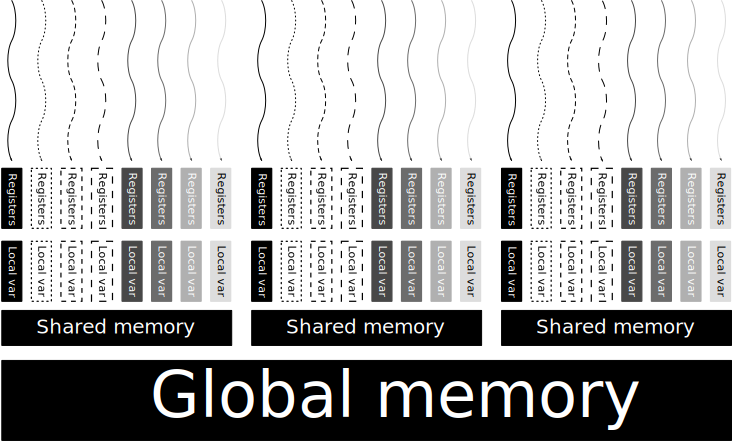
\includegraphics[scale=0.60]{Chapters/chapter1/figures/memory_hierarchy.pdf}}
\caption{Memory hierarchy of a GPU.}
\label{ch1:fig:memory_hierarchy}
\end{figure}



Shared memory allows  cooperation between threads of the  same block.  This kind
of memory is fast because it requires to be manipulated manually and its size is
limited.  It is accessible during the execution of a kernel. So the principle is
to fill the shared  memory at the start of the kernel  with global data that are
used very  frequently, then threads can  access it for  their computation.  They
can obviously change  the content of this shared  memory either with computation
or load of  other data and they can  store its content in the  global memory. So
shared memory can  be seen as a cache memory  manageable manually. This requires
obviously an effort from the programmer.

On  recent cards,  the programmer  may decide  what amount  of cache  memory and
shared memory is attributed to a kernel. The cache memory is a L1 cache which is
directly  managed by  the GPU.  Sometimes,  this cache  provides very  efficient
result and sometimes the use of shared memory is a better solution.




Figure~\ref{ch1:fig:memory_hierarchy}  illustrates  the  memory hierarchy  of  a
GPU. Threads are represented on the top  of the figure. They can access to their
own registers  and their local memory. Threads  of the same block  can access to
the shared memory of this block. The cache memory is not represented here but it
is local  to a thread. Then  each block can access  to the global  memory of the
GPU.

 \section{Conclusion}

In this chapter,  a brief presentation of the video card,  which has later been
used to perform computation, has been  given. The architecture of a GPU has been
illustrated focusing on the particularity of GPUs in term of parallelism, memory
latency and  threads. In order to design  an efficient algorithm for  GPU, it is
essential to have all these parameters in mind.


\putbib[Chapters/chapter1/biblio]

